% vim:textwidth=70
\chapter{基于日志的任务层次结构推断方法}
% XXX: model may not appropriate because no dependency
\label{chap:logmining}

\section{本章引言}

随着云计算逐渐影响人们的生活,分布式系统变的越来越重要,成了Internet应
用的关键组成部分~\cite{gfs, mapreduce, bigtable, dynamo}。分布式系统运
行在多台机器上,充分发掘并调度机器资源,以提供高吞吐率、低延迟的服务,
同时,还要处理各种不同类型的系统失败事件(failure)。由于系统规模庞大,
并且有严格的服务质量要求,设计与实现这类分布式系统不可避免的会产生错误
(bug),从而使系统表现出未预期的行为。系统错误的根本原因通常隐含在复
杂的应用逻辑之下,找到这些错误通常会花费很长时间。

理解分布式系统的运行时行为是验证系统设计、发现系统逻辑与性能问题、解决
系统实现错误的关键。然而,即使对系统的实现者来说,充分理解系统逻辑也不
是一件轻而易举的事情。这是因为,系统设计非常复杂,它的运行时行为多种多
样。再者,系统通常由一组程序员共同开发,并且在不停的演变至新的版本。进
一步说,分布式系统通常会使用分层的设计模式,将任务的执行过程分为不同层
次的阶段,其完成方式,可能是顺序的,也可能是并行的,跨越多个机器、进程
与线程。以上这些状况,都增加了理解系统运行时行为的困难。
% 用户请求由不同层次的模块处理。上层模块中的某个函数,会由下层模块的多
% 个函数一起完成,

已有的方法表明,用分层的任务模型去表达系统行为,可以很好的帮助程序员理
解与验证系统。例如,Pip~\cite{pip}允许程序员定义可嵌套的任务流,并定义
“期望”,来发现异常。用这个方法,程序员能够定义并验证系统特定层次的特
性。这种方法被证明能够很有效的发现系统错误与性能问题。我们之前的工作
Scalpel~\cite{scalpel}进一步发展了一种方法,能够从底层系统调用trace中,
自动推断任务模型,从而避免了手动定义任务结构的工作。初步的结果表明,从
操作系统层次的同步操作,我们能够推断出合理的表达上层语意的层次结构任务
模型。利用得到的模型,我们能够帮助程序员快速的发现并解决系统性能问题。

我们最终的目标是设计一个完全不需要或尽可能少需要人工标注的工具,来自动
提取系统的分层任务模型,帮助程序员、测试人员和系统管理员理解系统运行时
行为。基于之前的工作,在本文中,我们重点研究了如何利用系统日志(log)
来推断应用层任务的层次结构。相比底层trace,应用日志包含了更多的应用层
任务流的语意。日志是由系统开发人员创建的,因此它们包含了系统执行任务时
的关键参数与状态,例如,任务的类型,任务执行的关键步骤等等。这些信息可
以帮助我们推断应用层语意,而这些很难从系统调用trace中得到。

% 关键的系统状态和事件信息,例如,用户层任务的开始和结束,处理用户请求
% 的关键步骤等等。利用这些信息,

使用日志推断任务层次结构需要解决两个问题。第一、日志通常是非结构化的,
我们需要从中提取出和任务相关的信息。第二、推断任务之间的层次关系,从而
可以将系统活动分为层次结构的任务实例。

我们的解决方法是,首先,通过使用一组简单的启发,尽可能提取出日志中的任
务信息,包括任务的名称与ID。接着,依据任务ID的变化规律,推断任务的层次
关系。例如,我们可以在日志中发现这样的模式“request=R1,
operation=op1\yuanquan{a}\ldots \ldots request=R1,
operation=op2\yuanquan{b}\ldots \ldots request=R2,
operation=op3\yuanquan{c}”。request、operation是任务的名称,它们的值
表示相应任务ID。通过观察request任务ID的变化,我们可以推断R1任务的边界
在\yuanquan{a}处开始,在\yuanquan{c}之前结束,之间的日志条目都属于任务
R1,描述它的执行过程。进一步,任务是有层次关系的,同一个日志条目,可能
属于多个任务,通过观察多个任务ID的变化关系,我们可以推断不同任务之间的
层次关系。例如,同时考虑任务request和operation,我们发现,\yuanquan{a}
\yuanquan{c}之间的任务,同属于一个request任务R1,但是分属于不同的
operation任务,从而我们推断,request和operation任务之间,有层次嵌套关
系。通过对日志中所有的任务标识进行提取和推断,我们可以有效的推断出任务
之间的层次关系来。

我们实现了基于日志的任务层次结构推断工具,并使用它分析一个分布式存储系
统ChunkFS。ChunkFS是一个类似GFS~\cite{gfs}的分布式文件系统。我们的工具
能够推断出合乎逻辑的任务层次关系。应用得到的层次关系,能够帮助我们理解
ChunkFS的实际运行过程,并解决了ChunkFS中的一个性能问题。经验表明,系统
日志能够很好的反映出上层语意,我们的工具可以帮助理解系统设计和运行时行
为。

% XXX:文章组织

\section{推断方法设计}
\label{sec:lm_design}

图~\ref{fig:logmining_design}是推断方法设计概要。我们首先从无结构的系
统日志文本中提取出任务信息,并用(key, value)形式表示。key是任务名称,
value是任务ID。之后,我们推断key也就是任务之间的层次关系。我们利用得到
的任务层次关系分析系统动态行为。

% XXX: design flow

\begin{figure}
  \centering
  \begin{minipage}{0.8\linewidth}
    \centering
    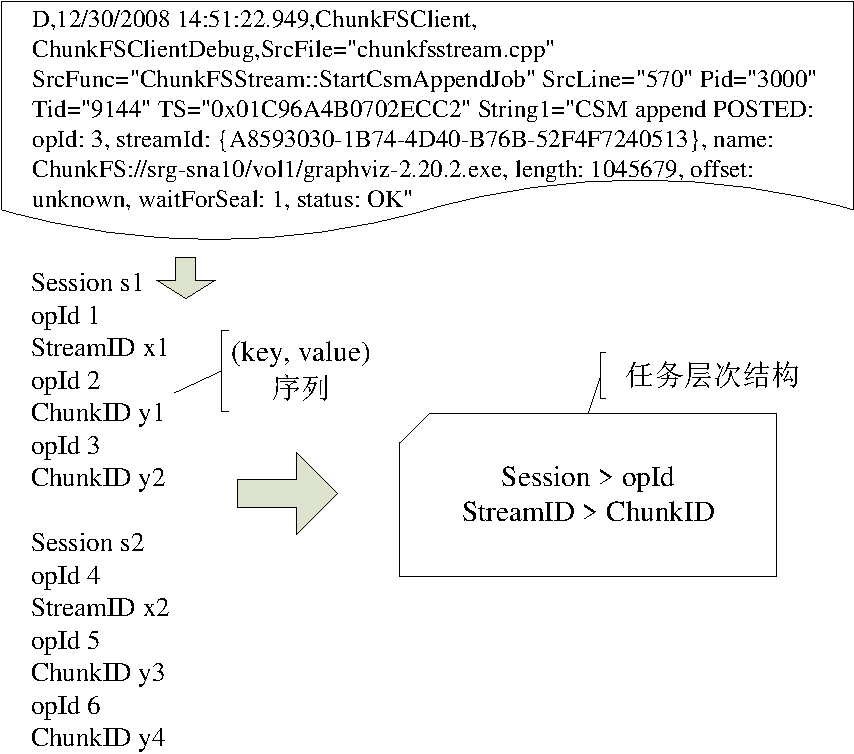
\includegraphics[width=1.0\linewidth]{mining_design}
    \caption{推断算法设计概要}
    \label{fig:logmining_design}
  \end{minipage}
\end{figure}

\subsection{提取任务信息}

日志包含了大量系统活动信息。我们需要从无结构日志文本中提取描述任务行为
与状态的信息。日志中包含的信息通常可以表达成为(key,value)对的形式。

图~\ref{fig:logmining_design}顶部是一个ChunkFS日志的例子。不同系统的日
志格式也不相同,ChunkFS的日志格式是一个典型代表。日志头的部分记录了日
志的级别、时间、类别,紧接着是所在文件、函数和行号,最后是进程号、线程
号。日志头是固定格式的。日志的后半部分,包含在Notes域里。它是程序员记
录的系统状态,包含了文字描述与数值表达的系统执行参数。任务信息通常都记
录在这里。

由于Notes中的内容是没有严格结构的,因此从中提取出(key,value)信息并
不容易。(key,value)在日志中通常被写成key SEP1 value SEP2的形式。其
中,SEP1是key和value的分隔符,SEP2是两个(key,value)之间的分隔符。
SEP1和SEP2的选择很多,可能是空格、逗号,分号等多种形式,并且不同的日志
条目会使用不同的SEP1、SEP2组合。key也有可能和文字描述中的单词是相同的
形式,例如图~\ref{fig:logmining_design}日志中的“POSTED:”和“opId:”。

我们使用对日志观察得到的启发,提取日志中的(key,value)信息。基于对日
志的观察,我们发现,value部分的格式是有限的,通常包括整数、十六进制数
和GUID,很容易使用正则表达式来匹配。一旦找到value部分,我们可以在文字
中向前跳过分隔符SEP1,遇到的第一个单词就是对应的key。

在少数情况下,value也可能是一个单词。但是目前我们只提取value为数值格式
的(key,value)对。这是因为,1)文字形式的value只是对某个状态的简单描
述,对于推断任务层次关系用处不大,2)由于SEP1和SEP2可能是空格,在这种
情况下,文字形式的value,会和key、其它文字混淆,无法区分。

\subsection{推断任务层次关系}

实际系统中的任务是有层次关系的,表现为任务执行过程的嵌套关系。一个高层
任务的执行,会被分解成为若干个低层任务。我们将任务之间的这种层次关系用
$>$表示,例如keyS$>$keyP,keyS、keyP是任务名称。经过提取任务信息步骤,
我们得到顺序的(key,value)任务信息序列,接下来,我们推断这个序列中
key之间的关系,并输出一组(keyS,keyP)二元组,表示keyS$>$keyP。

% 对每个线程分别推断?

% fig:keyvalue_sample

\begin{figure}
  \centering
  \begin{minipage}{0.8\linewidth}
    \centering
    \begin{lstlisting}[language=C++]
                    Session s1
                    opId 1
                    StreamID x1
                    opId 2
                    ChunkID y1
                    opId 3
                    ChunkID y2

                    Session s2
                    opId 4
                    StreamID x1
                    opId 5
                    ChunkID y1
                    opId 6
                    ChunkID y2
    \end{lstlisting}
    \caption{任务信息(key, value)序列示例}
    \label{fig:keyvalue_sample}
  \end{minipage}
\end{figure}


我们首先给出一个(key,value)序列的例子,如图~
\ref{fig:keyvalue_sample},以利于读者理解推断算法。图~
\ref{fig:keyvalue_sample}摘取了从ChunkFS的客户端程序日志中提取的任务序
列片段,它的意义是:在任务Session s1中,处理了某个客户端命令,对stream
x1进行操作,这些操作分成若干opId子任务执行,在opId 1中,首先进行了
stream层次的操作,例如打开或创建一个stream,之后,opId 2/3对stream的不
同chunk进行操作。

% stream,chunk是什么

我们使用如下两条规则从(key, value)序列中推断任务之间的层次关系,它们
是两个任务有$>$关系的充分必要条件。

\begin{itemize}

  \item 规则一:如果keyS$>$keyP,那么在(key, value)序列中,keyS的第一
  次出现早于keyP的第一次出现。

  \item 规则二:如果keyS$>$keyP,那么keyS的值域与keyP的值域,有严格的
  一对多关系,也就是一个父任务可以包含多个子任务,一个子任务,只能属于
  一个父任务。

\end{itemize}

通过规则一,我们可以判断任意两个任务可能存在的$>$关系。通过规则二,我
们使用(key,value)序列的数据,归纳任何两个keyS和keyP值域之间的映射关
系,从而得到任务之间的层次关系。

推断算法详细描述如下。算法扫描(key,value)序列,每读入一个
(key,value)对,就顺序更新三个数据结构。第一,每个key最新的value。第
二,一个key数组,维护key的首次出现顺序的关系,与规则一对应。数组中任何
一个key,都是它后面key的潜在父任务。算法读入一个(key,value)对,如果
key不在key数组中,则将它加入数组尾部。第三,任意两个key它们值域(value)
的对应关系,与规则二对应。对每个扫描到的(keyP,valueP),将(valueS,
valueP)加入(keyS,keyP)的值域对应关系(用一个字典维护,字典的键值是
(keyS,KeyP),对应的值是(valueS,valueP)数组。),keyS是key数组中
所有keyP前面的任务(即keyP的潜在父任务),valueS、valueP是keyS、keyP的
当前值。

这样,当扫描完(key,value)序列所有数据后,我们得到每一对(keyS,keyP)
的值域对应关系。应用规则二,判断是否keyS和keyP的值域有严格的一对多关系。

对图~\ref{fig:keyvalue_sample}中的例子,应用上面描述的算法,可以得出,
StreamID$>$ChunkID,Session$>$opId。Session和StreamID之间没有层次关系,
因为多个Session可能对应相同的StreamID(s1$\to$x1,s2$\to$x1)。类似的
(Session,ChunkID),(opId,StreamID)和(opId,ChunkID)也没有层次
关系。

\subsection{构建分层任务实例}

经过上一步,我们得到了任务两两之间层次关系。将所有这些关系联系起来,得
到了所有任务之间的偏序关系,可以用一颗或多颗树来表达得到的偏序关系。每
一颗树都是一个任务层次结构模型。在树中,每个节点都是一个任务,在实际
执行过程中,这个任务的执行过程包含若干它的子任务。程序员可以选择任意一
个层次模型对系统进行分析。为表示清晰起见,若原有任务层次模型的树根是
RootTask,我们增加一个新的节点Runtime,令它为RootTask的父节点,表示系
统运行时行为,由若干RootTask构成。

例如,对图~\ref{fig:keyvalue_sample}可以得到两个层次模型,
Runtime$>$Session,Session$>$opId和
Runtime$>$StreamID,StreamID$>$ChunkID。

我们将任务层次模型应用在系统日志上,将系统运行时行为分为有层次的任务实
例,每个实例都由一组系统日志构成,描述一段时间内的系统活动。系统行为首
先从任务层次模型的树根开始,分为高层任务实例。每个任务实例开始于任务ID
被赋予一个新的值,结束于任务ID被赋予另外一个值之前。在每个任务实例内部,
被递归的分为更低层的任务实例。

% XXX 图~\ref{fig:taskhierarchy_sample}
\begin{figure}
  \centering
  \begin{minipage}{0.8\linewidth}
    \centering
    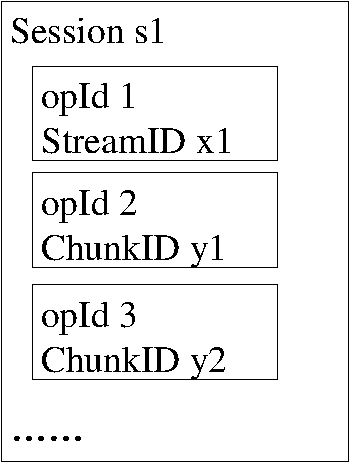
\includegraphics[width=0.4\linewidth]{mining_hierarchy}
    \caption{分层结构的任务实例}
    \label{fig:taskhierarchy_sample}
  \end{minipage}
\end{figure}


对于图~\ref{fig:keyvalue_sample}中的例子,我们应用Runtime$>$Session,
Session$>$opId任务层次模型,得到图~\ref{fig:taskhierarchy_sample}中的有层
次的任务实例。

分布式系统运行时包含若干运行在不同机器上的进程和线程,我们可以对每个线
程的日志分别提取任务信息、推断任务之间的层次关系,并将所有线程的任务层
次模型合并成为描述整个系统的层次模型。可以使用基于数值的join操作
(Magpie~\cite{magpie})将同一任务在不同机器、进程和线程的执行过程联系
到一起。

\section{讨论}
\label{sec:lm_discussion}

% 对提取出的(key,value)检查时,我们发现,由于程序员创建日志时未对key
% 的命名作严格约定,会产生下面问题:1)同一个key会有多个别名,2)不同的
% key可能使用相同的名字(key冲突)。我们使用命名映射同时解决了这两个问题。
% 在解析完一个日志条目后,会依据映射规则,把某些key转换为新名字。
% 
% 映射规则的形式如(FileX, FuncY, key) xxx (newkey),表示如果一个日志
% 条目的所属文件、函数是FileX、FuncY,那么将这个条目中的key转换为新的名
% 字newkey。FileX, FuncY可以使用正规表达式。这样,key别名可以用(*, *,
% alias) xxx (key)映射规则解决,而key冲突问题可以用(FileX, FuncY,
% conflict key) xxx (newkey)映射规则解决,从实际经验看,通常只需要指
% 明FuncY就可以解决冲突。

通常来说,并不是每个从日志中提取出的(key,value)对都描述任务信息,例
如key是error时,它描述的是某个任务执行的错误码。如果程序员对系统有一定
了解,可以从key的集合中选取出描述任务执行的key来,也就是任务名称。这有
两种情况。第一,key直接就是任务的名称,描述了某一类具有应用层语意的任
务,例如Session。第二,key是与任务一一对应的请求或数据。例如key是
requestID或eventID,表示目前正在处理的请求或事件是requestID,因此可以
用requestID代表正在处理它的任务。

即使程序员对系统了解不深,不能正确选出描述任务执行的key,我们的推断算
法仍然能帮助推断出任务层次结构来。程序员可以将所有(key,value)对不加
筛选的输入推断算法,推断算法能够筛选掉不存在$>$关系的(keyS,keyP)对,
给出可能存在$>$的(keyS,keyP)对。举例来说,如果将包含Session和error
的(key,value)序列输入推断算法,由于不同Session执行的错误码可以相同,
因此推断算法不会认为Session和error构成$>$关系。同时也存在不具有$>$关系
的key会被推断算法误判的情况。考虑Session和time的例子,time表示Session
开始执行的时间戳。由于不同Session执行的时间不相同,因而Session和time的
值域实际上存在一对一的关系,因此会被推断算法错误的认为存在$>$关系。因
此,将所有(key,value)对不加筛选的输入推断算法得到的结果是包含着误判
(false positive)但是不存在漏判(false negative)的结果。程序员可以将
推断的结果,与实际系统设计对比,筛去错误的结果,选出正确的结果。

% 正确的判别key是否描述任务信息,需要理解key的语意。我们采用了半自动的
% 方法来解决这一问题,首先,使用正则表达式,筛选掉肯定不表达任务信息的
% key,例如*size*, *err*, *offset*,接下来,请系统开发人员选出正确的
% key集合。采用这种方法,我们能够筛选掉大部分的不表达任务信息的key,从
% 而降低了开发人员的工作。

% 我们认识到,正确判断两个key是否有层次关系依赖于是否有足够多的数据,
% 使得不存在层次关系的key使用规则二被筛选掉。通常情况下,系统日志都足
% 够大,包含充分的数据,能够正确判断key的层次关系。

% 不同的人会怎么用推断工具

\section{应用实例}
\label{sec:lm_case}

% 是否能有效的提取key value

% 是否能有效挖掘出key的嵌套关系,挖掘出的关系好用不好用

% 应用得到的关系,能够帮助理解系统运行时行为,和调试性能问题

% logmining可以被不同的人使用。% xxx

在这一节,我们报告使用~\ref{sec:lm_design}节中的推断算法,从ChunkFS日
志中提取任务层次结构,并应用层次结构理解ChunkFS动态行为。同时,我们也
描述了,如何利用任务结构,解决系统的性能问题。

\subsection{理解系统运行时行为}

ChunkFS是一个分布式存储系统,它类似于GFS。ChunkFS由一个master和若干个
chunkserver构成。在ChunkFS中,数据被组织成一个个stream,对应GFS中的文
件概念。每个stream,由若干chunk构成。每个stream和chunk都有唯一的GUID标
识。我们在集群环境下部署一个ChunkFS实例,包含一个master,两个
chunkserver。我们向ChunkFS中随机的上传了若干文件,在上传命令之间,还随
机插入了若干查询命令,获取已上传文件的属性。ChunkFS运行的机器配置是:
2.0 GHz Xeon双核CPU,4 GB内存,运行Windows Server 2003 SP2操作系统,机
器间通过1 Gb网络连接。

% 若干文件?

首先分析ChunkFS客户端行为。我们发现ChunkFS客户端运行时有两类线程:一个
client线程和四个个worker线程。Client线程的任务模型是Runtime$>$Session,
Session$>$opId,worker线程的任务模型是Runtime$>$opId。

Client线程接收用户命令,每个用户命令,由一个新的Session任务执行,
Session任务被分为若干步骤,每一步是一个opId任务。在一个opId中,会发起
一到多个RPC调用,client线程并不直接调用RPC命令,而是将这个调用放入一个
RPC队列。Worker线程从RPC队列中取出RPC命令,并调用它们。当RPC命令返回时,
worker线程使用回调函数向client线程报告RPC调用的结果。对worker线程来说,
它们的行为被分为若干opId任务。Client线程和worker线程通过相同的opId联系
到一起。

我们详细的观察了上传文件至ChunkFS的过程,如图~
\ref{fig:chunkfs_client}所示。在客户端,创建新stream命令涉及一个
Session和4个opId,有6个RPC调用,具体过程是(create\_stream),(
append\_stream,append\_chunk),(append\_chunk),(append\_chunk,
seal\_chunk)。每个括号代表一个opId任务,括号内是RPC调用。由于文件小于chunk
大小的最大值,创建的stream只有一个chunk,其内容由3次append chunk RPC调
用写入。在最后一次append chunk RPC调用之后,chunk被封装,即seal\_chunk
RPC调用,之后,chunk不能再能够被写入或追加(append)。

\begin{figure}
  \centering
  \begin{minipage}{0.8\linewidth}
    \centering
    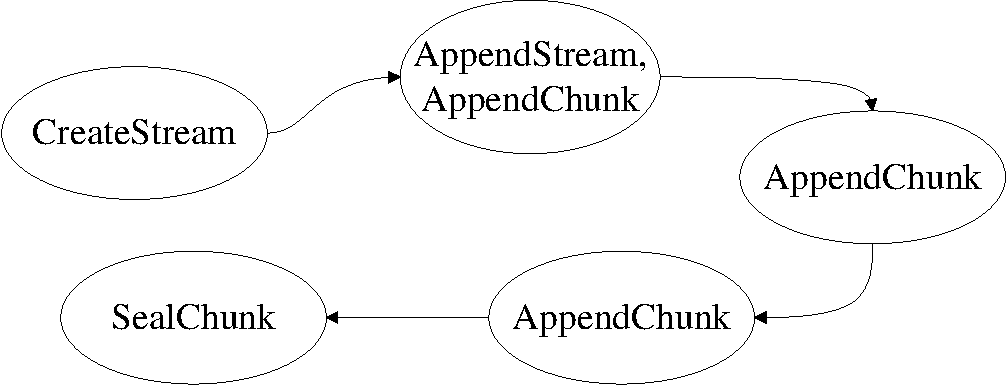
\includegraphics[width=\linewidth]{chunkfs_client}
    \caption{创建一个Stream操作,ChunkFS客户端client线程运行时行为。
    每个圆圈代表一个opId任务,整个四个圆圈代表一个Session任务}
    \label{fig:chunkfs_client}
  \end{minipage}
\end{figure}
% \ref{fig:chunkfs_client} 图表 4 创建一个Stream操作,ChunkFS客户端运
% 行时行为。每个圆圈代表一个opId任务,整个四个圆圈代表一个Session任务


我们同时观察在主chunkserver的运行时行为。Chunkserver端运行时包括若干线
程,其任务模型是Runtime$>$ChunkID。具体的,创建一个stream,Chunksever
会接到5个RPC调用,如图~\ref{fig:chunkserver}所示,分别是create\_chunk,
3个append\_chunk和seal\_chunk。可观察到的chunkserver行为的粒度被限制在对
chunk操作的级别(ChunkID任务),因此5个RPC处理被认为是同一个任务实例。

\begin{figure}
  \centering
  \begin{minipage}{0.8\linewidth}
    \centering
    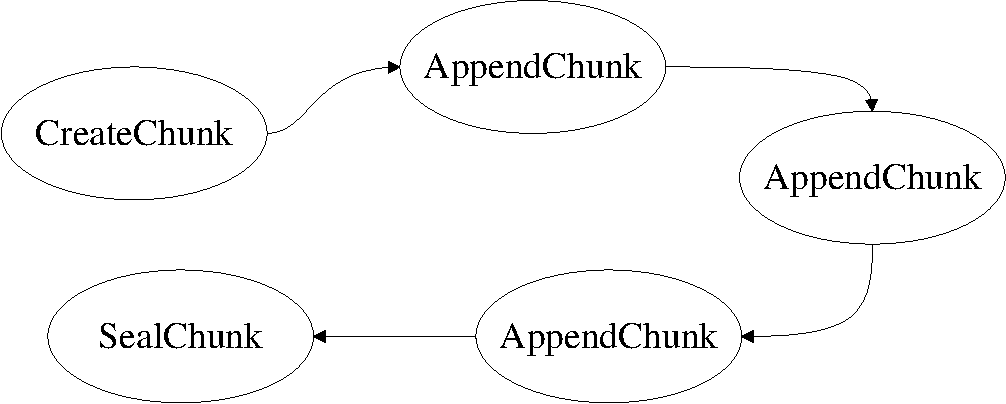
\includegraphics[width=\linewidth]{chunkfs_en}
    \caption{创建一个Stream操作,ChunkFS Chunkserver运行时行为。
    5个RPC被当作一个ChunkID任务,因为它们都对同一个Chuck进行操作}
    \label{fig:chunkserver}
  \end{minipage}
\end{figure}


% \ref{fig:chunkserver}图表 5创建一个Stream操作,ChunkFS Chunkserver运
% 行时行为。5个RPC被当作一个ChunkID任务,因为它们都对同一个Chuck进行操
% 作。

\textbf{经验}:使用任务模型,我们可以把系统运行时活动分为不同层次的任
务实例,有效的理解系统行为。任务层次结构实际上是隐含在系统设计中的,因
此利用任务模型从上至下的分解系统活动是有效的。

我们注意到,使用任务模型,也会产生一些不精确的地方。第一、任务边界可能
会有位移。通常任务都有一个初始化步骤,在这期间,任务标识可能还没有产生,
因此使用任务标识的变化来确定任务边界,会把初始化部分划分到上一个任务的
尾部。考虑到初始化部分通常是比较固定的若干步骤,可以对任务边界增加一个
修正量,解决这一问题。第二、任务的粒度依赖于任务层次结构的粒度,而后者
取决于日志中记录的任务信息。例如在先前的chunkserver例子中,5个RPC是五
个不同的任务,但是由于从日志中只能得到Runtime$>$ChunkID模型,所以会被
认为是同一个任务。

\subsection{解决系统性能问题}

使用任务模型可以帮助解决系统的性能问题。通过对ChunkFS测试,我们发现它
的网络函数库的性能指标不能达到要求。在一项压力测试中,在客户端,我们使
用10个并行线程,不断发起大小固定的文件上传任务。我们发现,无论如何改变
测试参数(并行线程数、上传文件大小),也不能够完全占用网络带宽,只有最
大值的35\%左右,同时CPU使用率也不到100\%。

根据我们先前的经验,系统性能问题,通常由于复杂的应用逻辑所引起,其根源
隐藏在庞大的代码库中。我们使用任务模型寻找产生性能问题的原因,并帮助定
位产生问题的代码。

我们重复了之前的压力测试,并收集任务相关的时间信息和资源使用情况。我们
确认了网络带宽和CPU资源都远远不能被充分利用。通过使用前面提到的client
线程和worker线程的任务模型,可以将上传文件操作区分为不同的opId任务。由
于网络数据传输主要由append\_chunk产生,因而可以认为每次opId任务近似等
于一次RPC调用。

% xxx: profiling process

图~\ref{fig:rpc_client}显示了client线程运行过程。10个Client线程不断的创建
RPC调用,并将它们放入一个共享队列,4个worker线程从队列中取出RPC调用,
并执行RPC,显示在图~\ref{fig:rpc_worker}
 
% \ref{fig:client} \ref{fig:worker}
\begin{figure}
  \centering
  \begin{minipage}{0.8\linewidth}
    \centering
    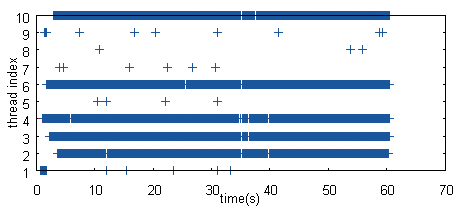
\includegraphics[width=\linewidth]{rpc_client.png}
    \caption{client线程创建RPC过程}
    \label{fig:rpc_client}
  \end{minipage}
\end{figure}

从图上立刻可以发现。Worker线程的执行过程呈现出被序列化的现象。虽然有4
个worker线程,但是他们调用RPC的任务的过程没有重叠,每一个时刻,只有一
个worker线程在工作。通过检查worker线程的设计与编码,我们发现了问题的根
源。为了使系统具有可扩展性(extensibility),worker线程不直接调用RPC,
而是使用processor对象去处理RPC调用。Processor对象是在worker线程间共享
的,并且对每个TCP连接只创建一个processor对象。因此,processor对象成为
了资源瓶颈,由于它只有一个,导致了若干worker线程被迫以序列化的方式工作。

\begin{figure}
  \centering
  \begin{minipage}{0.8\linewidth}
    \centering
    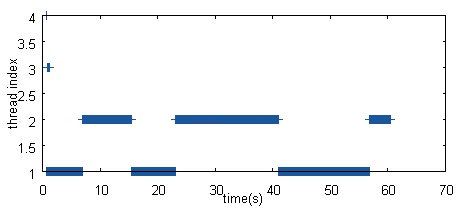
\includegraphics[width=\linewidth]{rpc_worker.png}
    \caption{worker线程执行RPC过程}
    \label{fig:rpc_worker}
  \end{minipage}
\end{figure}

\textbf{经验}:任务模型在帮助推断、解释系统问题时非常有用。通过分析任
务之间的依赖关系,共享资源(包括CPU、I/O,共享数据、变量、锁等)的使用
情况,可以有效的推断由资源冲突引起的系统性能问题。

\section{本章小结}
\label{lm_conclusion}
